\documentclass[11pt,onecolumn]{article}

\usepackage[margin=1in]{geometry}
\usepackage{amsmath,amssymb,amsthm}
\usepackage{graphicx}
\usepackage{bm}
\usepackage{booktabs}
\usepackage{array}
\usepackage{microtype}
\usepackage[colorlinks=true,linkcolor=blue,citecolor=blue,urlcolor=blue]{hyperref}
\usepackage{bookmark}
\hypersetup{
  pdftitle={The precision cost of temperature compensation in biochemical clocks: internal structure and dynamical activity, not entropy production},
  pdfauthor={Ricardo Romero},
  pdfsubject={Temperature compensation, stochastic biochemical clocks, phase-type renewal processes},
  pdfkeywords={temperature compensation, biochemical clocks, stochastic thermodynamics, phase-type distributions, dynamical activity}
}
\usepackage{authblk}
\usepackage{siunitx}

\newtheorem{proposition}{Proposition}
\newtheorem{theorem}{Theorem}
\newtheorem{lemma}{Lemma}
\newtheorem{corollary}{Corollary}
\theoremstyle{definition}
\newtheorem{definition}{Definition}
\newtheorem{result}{Result}
\newtheorem{remark}{Remark}

\newcommand{\CV}{\mathrm{CV}}
\newcommand{\Ncoh}{\mathcal{N}}
\newcommand{\Aact}{\mathcal{A}}
\newcommand{\Keq}{K_{\mathrm{eq}}}
\newcommand{\Emax}{E_{\max}}
\newcommand{\dd}{\mathrm{d}}
\newcommand{\ee}{\mathrm{e}}
\newcommand{\Tzero}{T_0}
\newcolumntype{L}[1]{>{\raggedright\arraybackslash}p{#1}}

\title{\bfseries The precision cost of temperature compensation in biochemical clocks: internal structure and dynamical activity, not entropy production}

\author[1]{Ricardo Romero\thanks{\texttt{rromero@cua.uam.mx}}}
\affil[1]{Departamento de Ciencias Naturales, Universidad Aut\'onoma Metropolitana--Cuajimalpa, Mexico City, Mexico}

\date{\today}

\begin{document}
\maketitle

\begin{abstract}
\noindent
Most circadian clocks hold a nearly temperature-independent period despite being built from strongly temperature-dependent elementary rates. This is classically explained by an antagonistic balance of activation energies weighted by control coefficients (Ruoff), and more recently by \emph{period-lengthening reactions} operating far from onset, at a cost in free-energy dissipation (Fu \emph{et al.}). Because the coherence of a stochastic oscillator is thermodynamically bounded (Barato--Seifert), it is natural to ask whether temperature compensation (TC) carries a cost in the complementary currency of oscillator precision. Working with renewal (phase-type) clock models, we report five results and delimit their scope explicitly. (i) A kinematic necessity: within Arrhenius kinetics, compensation requires at least one period-lengthening reaction, and a purely sequential clock cannot compensate (Proposition~\ref{prop:positivity}). (ii) For a \emph{canonical minimal} single-excursion mechanism, the compensated coherence obeys an exact trade-off with an $N$-independent floor $1/\pi$ (Result~\ref{res:single}); we also note that the canonical memoryless compete-or-advance version is overdispersed, $\CV^2\ge 1$. (iii) This trade-off is not universal: an entropic-gating construction achieves compensation with squared coefficient of variation $\CV^2 = 1/m$ \emph{independent} of the required temperature sensitivity, so precision and compensation decouple (Result~\ref{res:nofloor}). (iv) For the two-state gate, an exact finite-equilibration law $\CV^2=\tfrac{1}{m}(1+2\epsilon\Keq/(1+\Keq))$ and an exact identity $(\CV^2_{\mathrm{step}}-1)\,\Aact_{\mathrm{step}}=4\Keq^2/(1+\Keq)^2$ show the residual cost, in this construction, appears as dynamical activity rather than entropy production (Result~\ref{res:activity}). (v) For order-$n$ Arrhenius phase-type dwells with an activation-energy budget, a sandwich $1/n \le \CV^2_{\min}(n,R)\le 1/(n-1)$ (Theorem~\ref{thm:sandwich}) bounds the coherence cost of compensation to less than one effective step, vanishing relative to the ceiling as $n\to\infty$. In the model classes analyzed here, compensation therefore need not require increased entropy production; the remaining cost appears as internal-state complexity and dynamical activity---both genuine physical resources. This predicts that clocks that are simultaneously precise and well compensated should implement compensation through multi-state, entropically-gated modules rather than single competing reactions, consistent with the large, multi-conformational KaiC ATPase; concrete experimental tests are tabulated. The exact constrained optimum $\CV^2_{\min}(n,R)$ is left as a well-posed extremal phase-type problem.
\end{abstract}

\section{Introduction}

Circadian and other biological clocks maintain a period that is remarkably insensitive to temperature, even though the underlying enzymatic rates are Arrhenius-activated and individually change several-fold over the physiological range. The cleanest experimental exemplar is the reconstituted cyanobacterial KaiABC oscillator, a temperature-compensated post-translational rhythm driven by ATP hydrolysis \cite{Nakajima2005}; the rate-limiting KaiC ATPase turns over only $\sim 15$ ATP per day and is itself nearly temperature-invariant, and its turnover sets the clock frequency \cite{Terauchi2007}.

The classical account of temperature compensation (TC) is Ruoff's \emph{antagonistic balance} \cite{Ruoff1992}: writing each rate in Arrhenius form $k_j = A_j\,\ee^{-E_j/T}$ (we set $k_B=1$ throughout), the period $\tau(\{k_j\})$ is compensated when
\begin{equation}
\frac{\dd \ln\tau}{\dd T} = \frac{1}{T^2}\sum_j C_j E_j = 0,
\qquad
C_j \equiv \frac{\partial\ln\tau}{\partial\ln k_j},
\qquad
\sum_j C_j = -1,
\label{eq:ruoff}
\end{equation}
where the $C_j$ are the period control coefficients obeying the metabolic-control summation theorem \cite{Wu2017,RuoffWesterhoff2007}. Fu, Fei, Ouyang and Tu showed from a general timescale invariance that TC relies on the existence of \emph{period-lengthening reactions}, whose rates \emph{increase} the period, and that this typically requires operating far from the Hopf onset; they further reported that better TC performance requires higher energy dissipation \cite{Fu2024}.

The precision of a stochastic oscillator is itself thermodynamically constrained: the number of coherent oscillations is bounded by the driving affinity and network topology \cite{BaratoSeifert2017,Oberreiter2022}, the free-energy cost of accurate biochemical oscillations is finite \cite{Cao2015,Fei2018}, and Brownian clocks obey a cost--precision trade-off \cite{BaratoSeifert2016}. With a dissipation cost of TC on one side and a dissipation bound on precision on the other, it is natural to ask whether TC carries a cost in the currency of coherence itself.

We find that the intuitive ``compensation costs precision'' expectation holds only for the structurally simplest mechanisms and dissolves once the compensating element is allowed internal structure. The mechanism-independent invariant is only the kinematic necessity of a period-lengthening reaction; the actual costs of compensating \emph{well} are structural (internal states, activation-energy contrast) and kinetic (dynamical activity), and are bounded to within a factor $n/(n-1)$ of free. We separate throughout exact, general statements from results proven for specific canonical constructions, and we use ``dissipation'' to mean steady-state entropy production, reserving ``dynamical activity'' for the (distinct) kinetic traffic that appears as the residual cost.

\section{Renewal clocks: period, coherence and the compensation deficit}
\label{sec:setup}

We model a clock as a renewal process whose ``tick'' is the completion of a productive cycle of $N$ stages. Each stage $i$ has an independent dwell time with density $\psi_i$, mean $\mu_i$ and variance $v_i$; the cycle time $T_{\mathrm{cyc}}=\sum_i T_i$ has
\begin{equation}
\tau \equiv \langle T_{\mathrm{cyc}}\rangle = \sum_i \mu_i,
\qquad
\mathrm{Var}(T_{\mathrm{cyc}}) = \sum_i v_i .
\end{equation}
We use two coherence measures. For a finite Markov generator the standard measure is the eigenvalue coherence $\Ncoh_{\mathrm{eig}}=|\mathrm{Im}\,\lambda_1|/|\mathrm{Re}\,\lambda_1|$ of the oscillatory clock mode \cite{BaratoSeifert2017}; in the finite two-loop sweep of Fig.~\ref{fig:trade}, this mode is tracked by the largest imaginary frequency to avoid switching to weakly damped spectator modes. For renewal (phase-type) dwells the natural measure is the phase-diffusion coherence
\begin{equation}
\Ncoh = \frac{1}{\pi}\,\frac{\tau^2}{\mathrm{Var}(T_{\mathrm{cyc}})}
= \frac{1}{\pi\,\CV^2},
\qquad
\CV^2 \equiv \frac{\mathrm{Var}(T_{\mathrm{cyc}})}{\tau^2},
\label{eq:Ndef}
\end{equation}
obtained from the accumulation of independent per-cycle timing jitter. The two agree up to an $O(1)$ prefactor: a uniform irreversible $N$-ring has $\Ncoh_{\mathrm{eig}}=\cot(\pi/N)$ and $\Ncoh = N/\pi$, which coincide asymptotically. Both are scale-invariant, so fixing the period costs nothing and $\Ncoh$ depends only on the \emph{shape} of the cycle-time distribution. Angular frequency is $\omega=2\pi/\tau$, and we quantify the residual temperature sensitivity of the period by the compensation deficit
\begin{equation}
\chi \equiv \left|\frac{\dd\ln\omega}{\dd T}\right| = \left|\frac{\dd\ln\tau}{\dd T}\right| .
\end{equation}
Perfect compensation is $\chi=0$.

\paragraph{Notation and conventions.} To avoid symbol collisions we fix: $N$ is the number of cycle stages / phase-type order; $m$ is the number of gated stages of a compensating module; $\Ncoh$ (calligraphic) is coherence, never a stage count; $\Keq=f/b$ is the \emph{equilibrium} occupancy ratio of a two-state trap (forward/backward trap rates $f,b$); $\epsilon=p/(f+b)$ is the trap-equilibration parameter ($p$ the productive advance rate); and $\Aact_{\mathrm{step}}$ (calligraphic) is the \emph{dynamical activity} of a gated step, defined as the expected number of \emph{directed} trap traversals (both $X\to Y$ and $Y\to X$) per completed step. Arrhenius rates are $k=A\,\ee^{-E/T}$ with prefactor $A>0$ and activation energy $E\ge 0$; the reference temperature is $\Tzero$.

\section{Kinematic necessity of a period-lengthening reaction}
\label{sec:positivity}

Equation~\eqref{eq:ruoff} shows that, since $E_j\ge 0$ and $\sum_j C_j=-1$, compensation ($\sum_j C_j E_j=0$) requires some control coefficient to be \emph{positive}: a reaction whose acceleration \emph{lengthens} the period. We sharpen this into a structural impossibility for sequential clocks.

\begin{proposition}[Positivity lemma]
\label{prop:positivity}
A clock whose cycle time is a sum of independent, forward-only Arrhenius stages cannot be temperature compensated: its period is strictly decreasing in temperature ($Q_{10}>1$), with all control coefficients negative.
\end{proposition}

\begin{proof}
For forward-only stages $\tau=\sum_j 1/k_j^+=\sum_j A_j^{-1}\ee^{E_j\beta}$ with $\beta=1/T$. Each term is strictly increasing in $\beta$, so $\dd\tau/\dd\beta=\sum_j E_j A_j^{-1}\ee^{E_j\beta}>0$, hence $\dd\tau/\dd T<0$. Moreover $\dd\ln\tau/\dd\beta = \langle E\rangle_w>0$ with positive Boltzmann-like weights $w_j=A_j^{-1}\ee^{E_j\beta}/\tau$, so every $C_j=-w_j<0$.
\end{proof}

Compensation therefore requires breaking the positivity of these weights, i.e.\ introducing a genuine period-lengthening element (a trap, branch or feedback with $C_j>0$), in agreement with \cite{Fu2024}. All subsequent sections concern the \emph{cost} of that element. Writing $\ln\tau(\beta)$ as the logarithm of a generalized partition function makes broadband compensation transparent: requiring $\dd\ln\tau/\dd\beta\approx 0$ over a temperature band forces successive $\beta$-cumulants of a \emph{signed} activation-energy measure to vanish, each an independent codimension-one condition, so broadband compensation is fragile unless a structural mechanism pins the cumulants---which is what the constructions below provide.

\section{A canonical single-excursion trade-off}
\label{sec:twoloop}

Consider the smallest driven oscillator with a period-lengthening element: a strongly driven productive $N$-ring (here $N=4$, coherence ceiling $\cot(\pi/4)=1$) whose node $0$ additionally opens a driven side-excursion sharing that node (Fig.~\ref{fig:trade}). Entering the excursion steals dwell time from ring progression---a negative frequency control coefficient---and because the excursion's entry has a higher activation energy than the ring, heating diverts more traffic into it, pulling the period back up: temperature compensation. Numerically, sweeping the excursion's competitiveness $g$ drives $\chi\to 0$ at a compensation point $g^\ast$ while the eigenvalue coherence falls monotonically (Fig.~\ref{fig:trade}A); the achievable region over all parameters shows a frontier of maximal coherence that slopes down as $\chi\to 0$ (Fig.~\ref{fig:trade}B). Notably the entropy production does \emph{not} rise at $g^\ast$---in this model it falls (Fig.~\ref{fig:trade}C)---so the cost here is paid in coherence, not dissipation.

\begin{figure}[t]
\centering
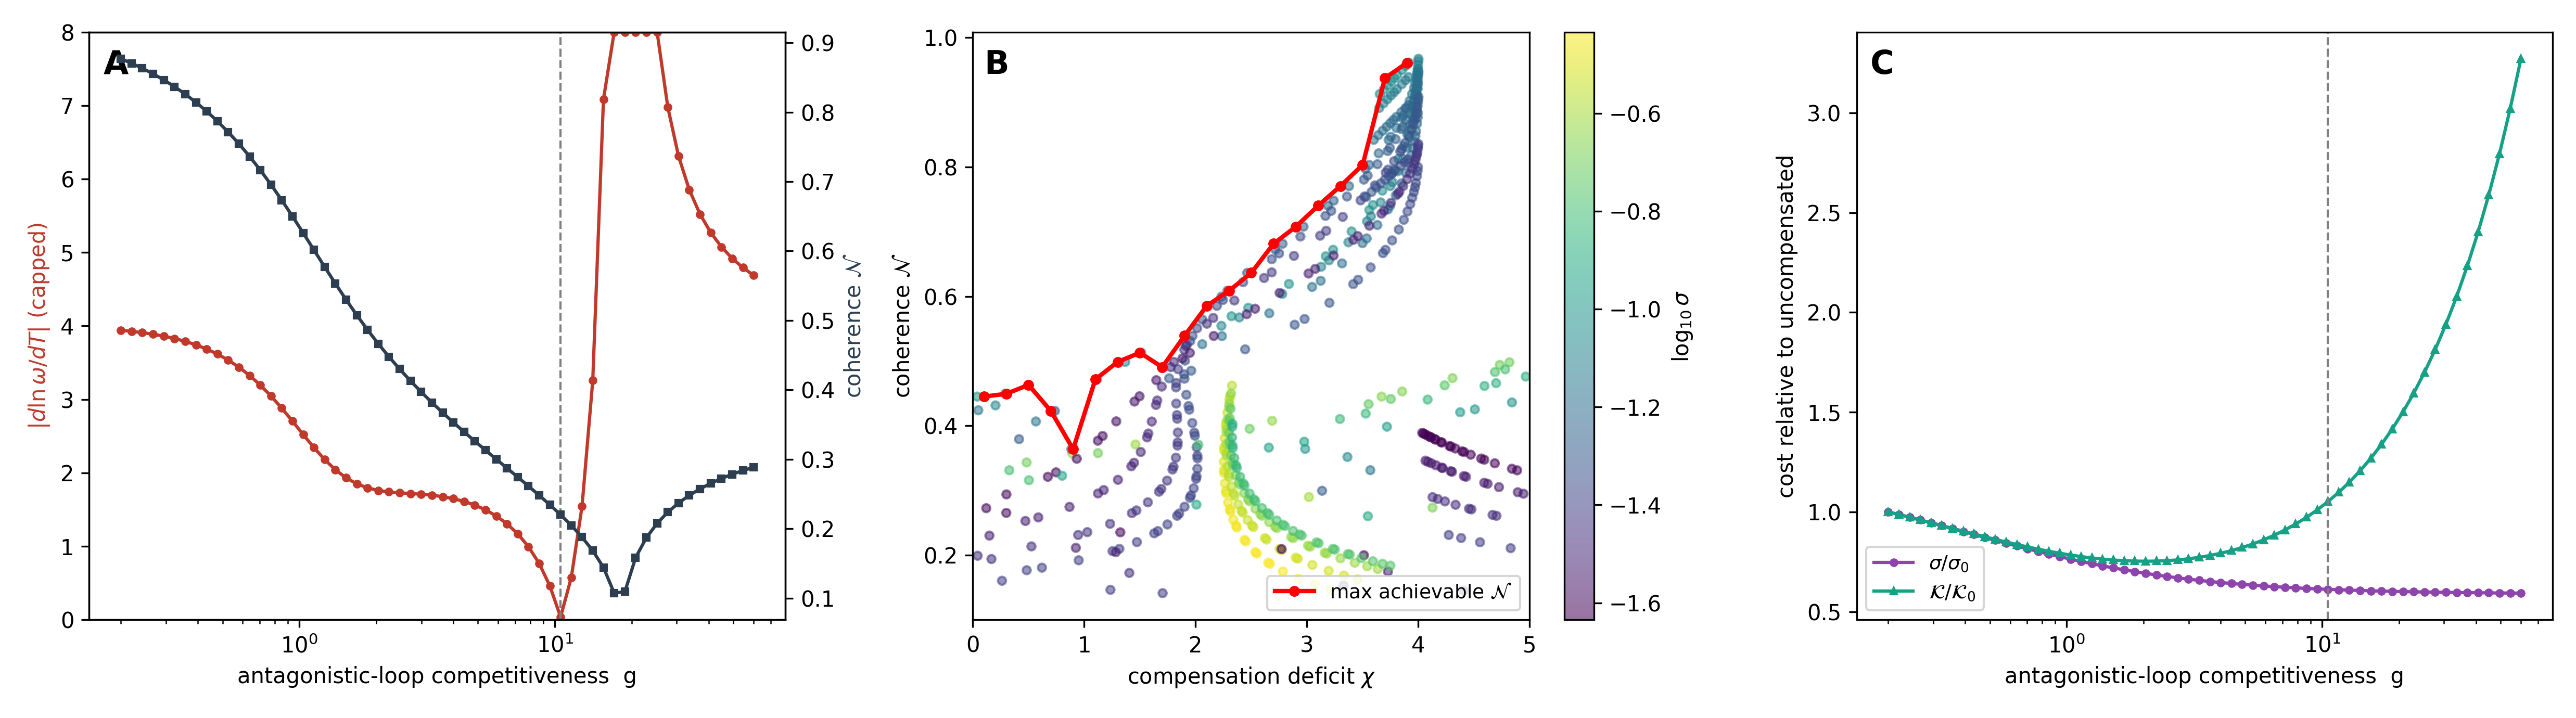
\includegraphics[width=\linewidth]{../figures/fig1_twoloop.png}
\caption{\textbf{Canonical single-excursion oscillator} (6-state model; productive ring $0\!\to\!1\!\to\!2\!\to\!3\!\to\!0$ with forward prefactor $1$, reverse prefactor $b_{\mathrm{ring}}=0.03$, ring activation $E_A=4$; side-excursion entry $0\!\to\!4$ with activation $E_B=9$ and prefactor $200g$; fast internal return $4\!\to\!5\!\to\!0$; $k_B=1$, $\Tzero=1$). \textbf{(A)} As the side-excursion competitiveness $g$ increases, the compensation deficit $\chi=|\dd\ln\omega/\dd T|$ falls to zero at $g^\ast$ while the clock-mode eigenvalue coherence $\Ncoh=|\mathrm{Im}\,\lambda_1|/|\mathrm{Re}\,\lambda_1|$ declines monotonically. \textbf{(B)} Achievable region over all parameters; the frontier of maximal coherence slopes toward $\chi\to0$. Colour is $\log_{10}$ of the steady-state entropy production $\sigma=\sum_{\mathrm{edges}}(J^+-J^-)\ln(J^+/J^-)$ (natural units, $k_B=1$). \textbf{(C)} Relative to the uncompensated baseline, entropy production $\sigma$ does not rise at $g^\ast$ (it falls to ${\sim}0.6\times$); dynamical activity $\mathcal{K}=\sum_{\mathrm{edges}}\pi_s k_{s\to d}$ is roughly flat until one over-drives past $g^\ast$.}
\label{fig:trade}
\end{figure}

This trade-off admits an exact closed form via a semi-Markov reduction (Appendix~\ref{app:derivations}). Collapsing the side-excursion into the waiting time of node $0$ gives the exact Laplace transform of the node-0 dwell,
\begin{equation}
\psi_0(s) = \frac{a}{\,a + s + d\,[1-\psi_e(s)]\,},
\label{eq:psi0}
\end{equation}
with $a$ the ring-advance rate, $d$ the diversion rate and $\psi_e$ the excursion transform (Appendix~\ref{app:A1}). For an exponential excursion of mean $\mu_e$ and, in units $a=k=1$, delay $\Delta=n_{\mathrm{ex}}\mu_e$ ($n_{\mathrm{ex}}=d/a$ the mean number of excursions), the cycle statistics are (Appendix~\ref{app:A2})
\begin{equation}
\tau = N+\Delta,
\qquad
\mathrm{Var} = N + 2\Delta + 2\mu_e\Delta + \Delta^2,
\qquad
\Ncoh = \frac{\tau^2}{\pi\,\mathrm{Var}} .
\label{eq:trapmoments}
\end{equation}
With Arrhenius rates (ring $E_A$, entry $E_B$, excursion $E_e$) the compensation condition $\dd\tau/\dd T=0$ yields (Appendix~\ref{app:A3})
\begin{equation}
\Delta^\ast = \frac{N E_A}{G},
\qquad
G \equiv E_B - E_A - E_e > 0,
\label{eq:comp}
\end{equation}
so compensation demands that the antagonist be \emph{more} temperature-sensitive than the advance and excursion steps combined. The best coherence compatible with compensation (low-variance limit $\mu_e\to0$) is (Appendix~\ref{app:A4})
\begin{equation}
\Ncoh^\ast = \frac{(N+\Delta^\ast)^2}{\pi\,(N + 2\Delta^\ast + {\Delta^\ast}^2)},
\label{eq:frontier}
\end{equation}
with two fuel- and dissipation-independent limits (Fig.~\ref{fig:closed}): the ceiling $N/\pi$ as $G\to\infty$ and a floor $\Ncoh^\ast \to 1/\pi$ as $G\to 0^+$, \emph{independent of $N$}.

\begin{figure}[t]
\centering
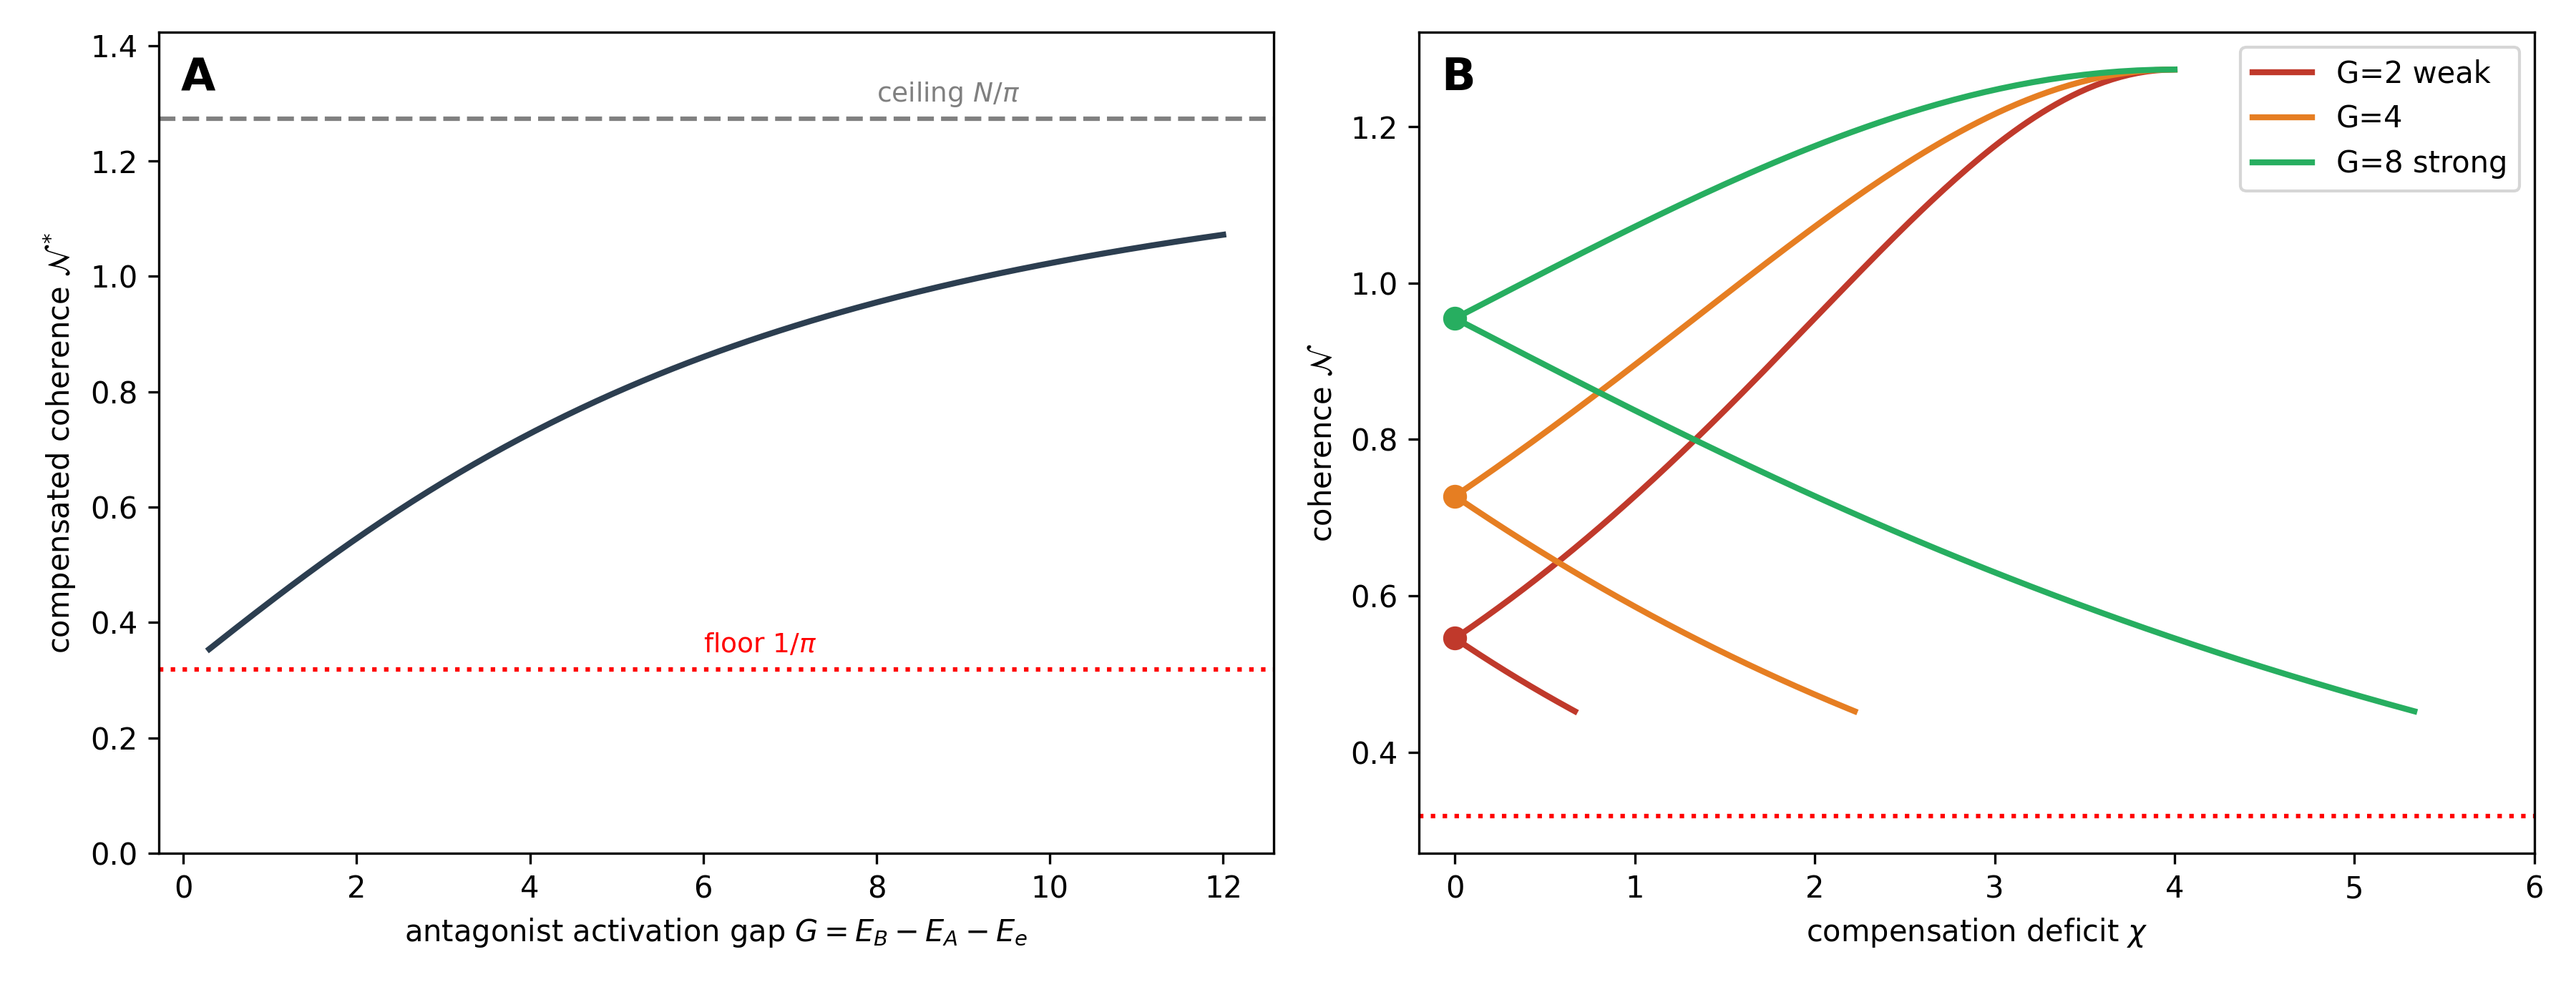
\includegraphics[width=0.92\linewidth]{../figures/fig2_closedform.png}
\caption{\textbf{Closed-form single-timescale result.} \textbf{(A)} Best compensated coherence $\Ncoh^\ast$ [Eq.~\eqref{eq:frontier}] versus the antagonist activation gap $G=E_B-E_A-E_e$, between the uncompensated ceiling $N/\pi$ and the $N$-independent floor $1/\pi$. \textbf{(B)} Frontier $\Ncoh(\chi)$ at fixed $G$; filled markers denote full compensation ($\chi=0$).}
\label{fig:closed}
\end{figure}

\begin{result}[Single-timescale trade-off, canonical mechanism]
\label{res:single}
For the canonical single-excursion (semi-Markov) mechanism of Eqs.~\eqref{eq:psi0}--\eqref{eq:frontier}, the compensated coherence is bounded by $\Ncoh^\ast(G)$, with an $N$-independent floor $1/\pi$ attained as the antagonist's temperature sensitivity vanishes.
\end{result}

\begin{remark}
The over-dispersion underlying Result~\ref{res:single} is a property of the canonical memoryless race-return construction, not a universal theorem. In that construction, the decision to advance (rate $p$) or divert through a competing route creates a mixture of dwell times and hence an overdispersed element with $\CV^2\ge 1$; more structured diverted routes can escape this only by adding internal states, which is precisely the mechanism developed below. The specific frontier~\eqref{eq:frontier} is therefore proven only for the construction above.''
\end{remark}

\section{Refutation of a universal trade-off: sub-Poissonian compensation}
\label{sec:refute}

Result~\ref{res:single} is tempting to promote to a universal law; it is not one. A numerical search over internal network structures readily finds period-lengthening elements ($\dd\mu/\dd T>0$) with $\CV^2$ well below unity, and constrained optimization pushes them to $\CV^2\approx 0.4$--$0.5$ even at strong sensitivity. The universal precision penalty does not exist.

The mechanism that evades it is an \emph{entropic gate}. Every Arrhenius rate increases with $T$, so an anomalous (period-lengthening) step cannot be built from a single rate; it requires an off-pathway trap that is entropically favoured but enthalpically costly, so that it becomes \emph{more} populated as temperature rises, throttling the effective forward rate. Concretely, replace each productive state $X_i$ (advance rate $p$) with a fast two-state pool $X_i\rightleftharpoons Y_i$ at rates $f,b$; fast equilibration renormalizes the step to an effective rate $k_{\mathrm{eff}}=p/(1+\Keq)$ with $\Keq=f/b=\exp(\Delta S-\Delta H/T)$ for an entropically favoured ($\Delta S>0$), enthalpically costly ($\Delta H>0$) trap. Thus $\Keq$ increases with $T$, so $k_{\mathrm{eff}}$ \emph{decreases} in $T$. Chaining $m$ such gated stages, the exact first-passage moments give (Appendix~\ref{app:A5})
\begin{equation}
\CV^2 \;\xrightarrow{\ \text{fast gating}\ }\; \frac{1}{m},
\end{equation}
\emph{independent} of the compensation strength $R\equiv\dd\ln\mu_0/\dd T$. The per-step sensitivity is set entirely by the trap enthalpy, $R = \tfrac{\Keq}{1+\Keq}\tfrac{\Delta H}{T^2} - \tfrac{E_p}{T^2}$, bounded only by the available activation-energy budget, $R \le R_{\max}\approx (\Emax-E_p)/T^2$. Coherence ($1/\CV^2=m$) and compensation strength ($R$ via $\Delta H$) are thus \emph{orthogonal} knobs (Fig.~\ref{fig:nofloor}).

\begin{figure}[t]
\centering
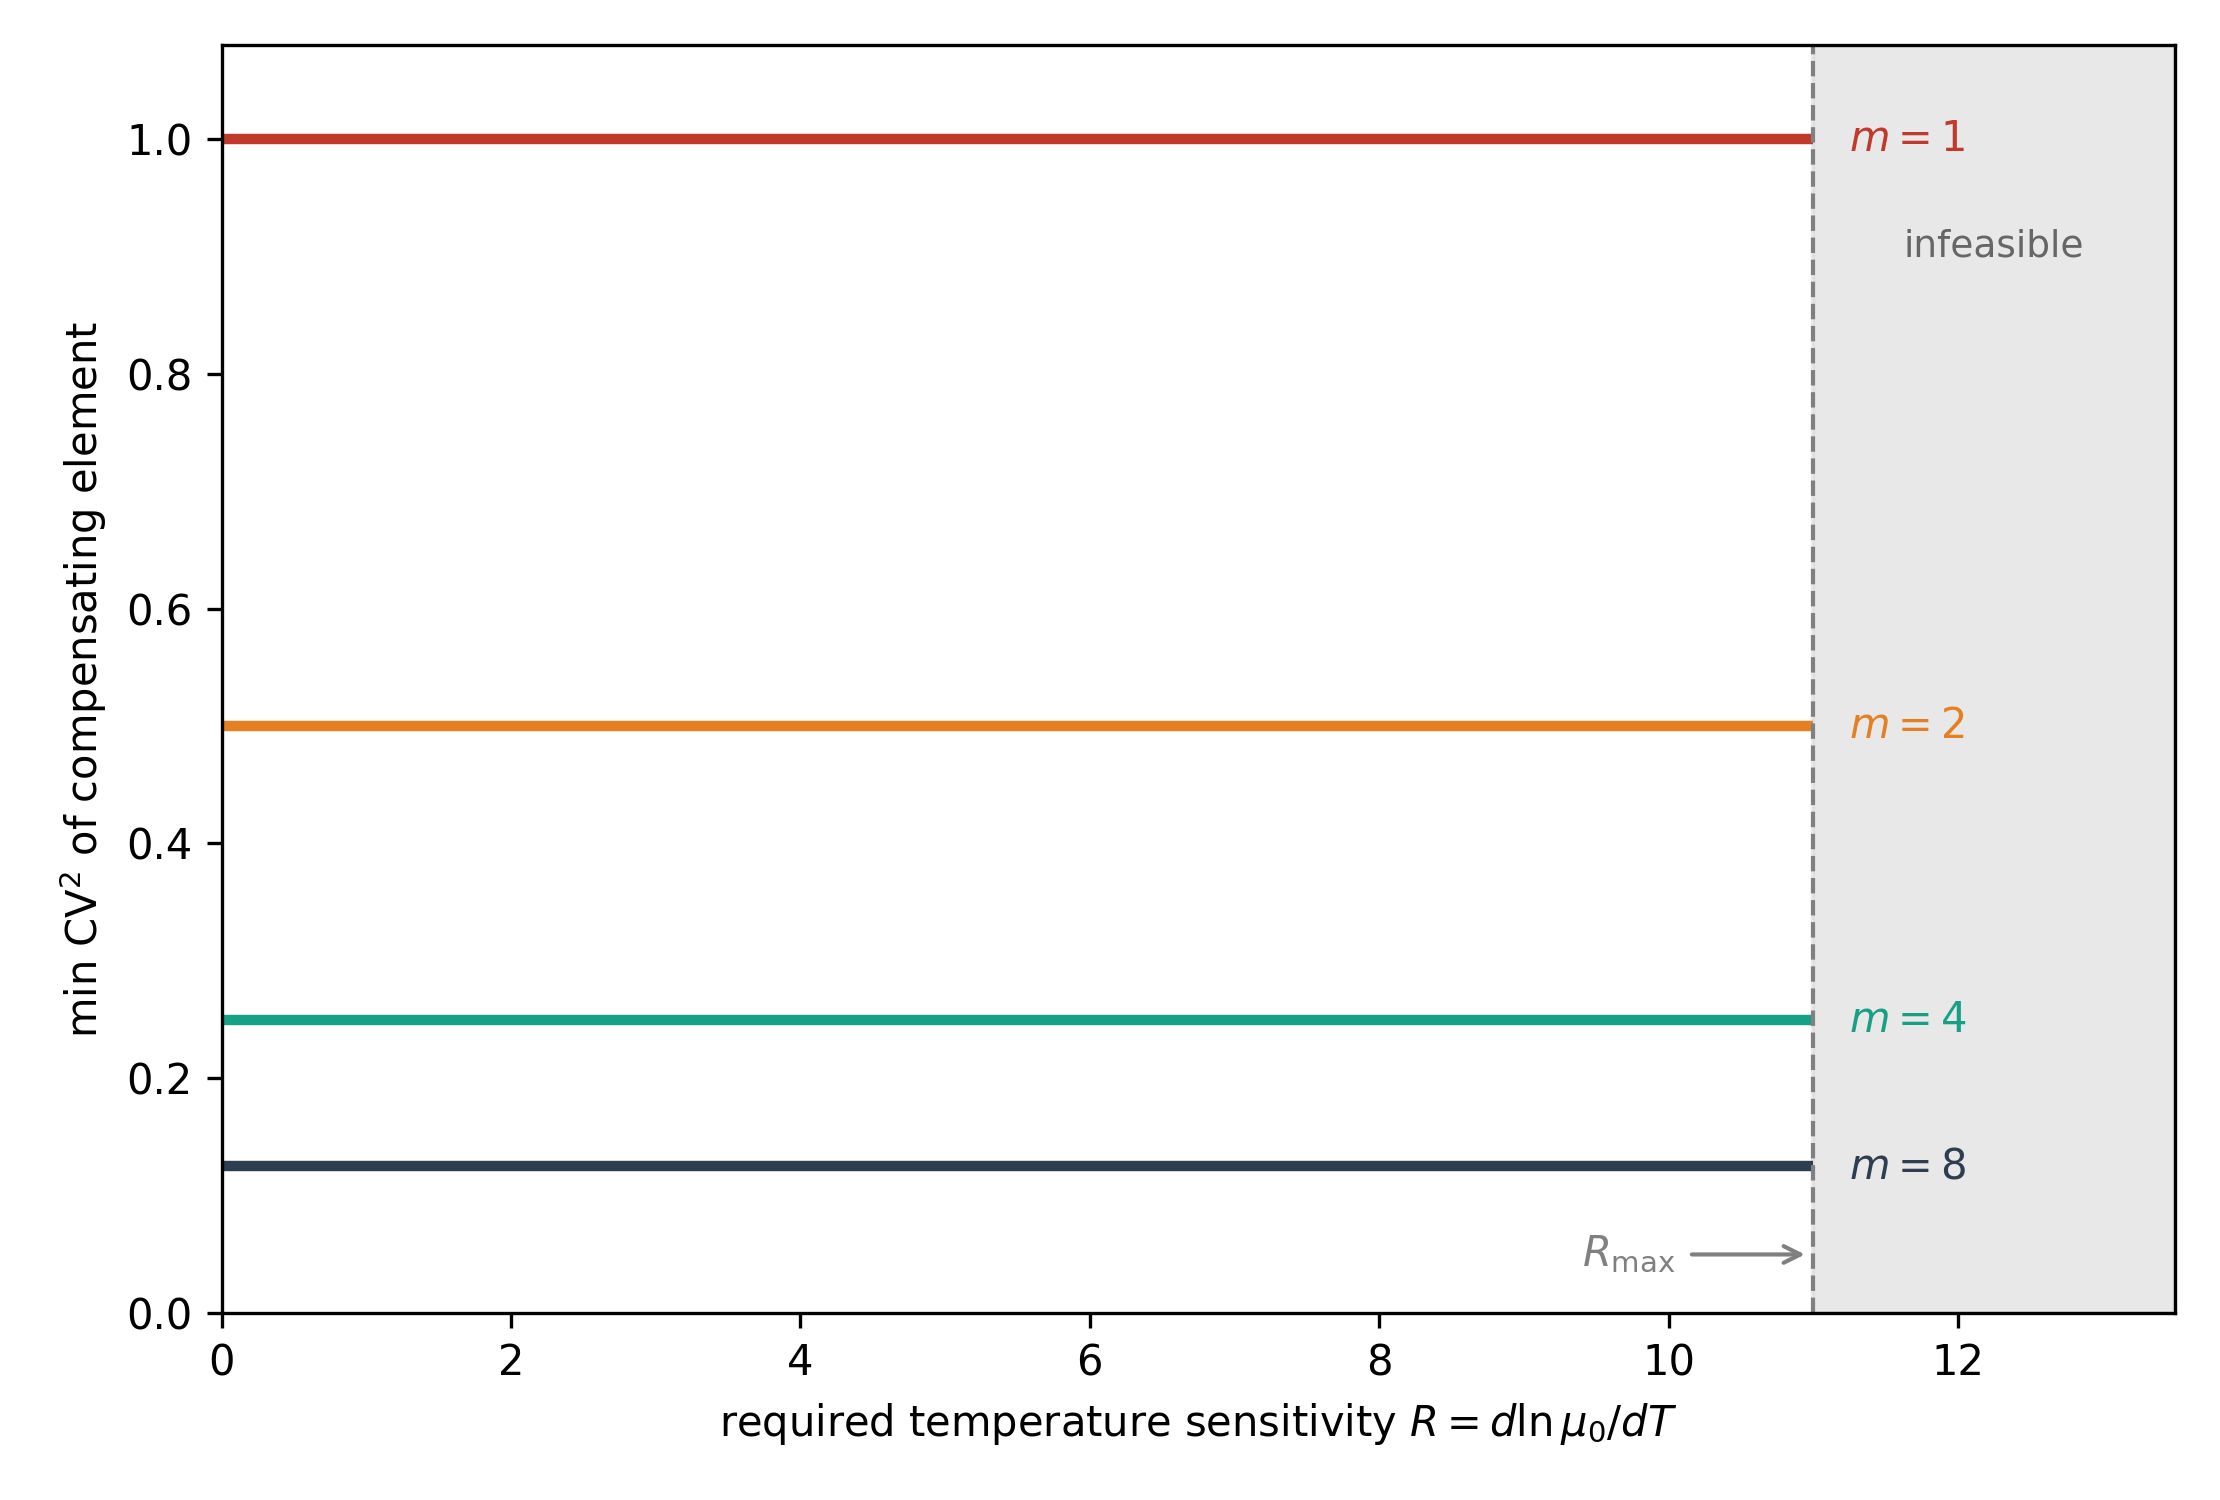
\includegraphics[width=0.7\linewidth]{../figures/fig3_nofloor.png}
\caption{\textbf{No precision penalty.} The minimum $\CV^2=1/m$ of an entropically-gated compensating chain is flat in the compensation strength $R$, up to the activation-budget ceiling $R_{\max}\approx(\Emax-E_p)/T^2$ (dashed; feasible region to the left). Coherence is set by the number of stages $m$; compensation strength by the trap enthalpy; the two are independent. Curves are the exact first-passage $\CV^2$ of the $2m$-state gated chain.}
\label{fig:nofloor}
\end{figure}

\begin{result}[No universal precision penalty]
\label{res:nofloor}
Temperature compensation carries no mechanism-independent coherence penalty: an entropically-gated chain of $m$ stages achieves $\CV^2\to 1/m$ in the fast-gating limit, independent of the required sensitivity $R$ up to the activation-energy budget.
\end{result}

\section{Finite-equilibration law and the activity identity}
\label{sec:finite}

The floor $1/m$ is the limit of instantaneous trap equilibration. For a finite equilibration parameter $\epsilon=p/(f+b)$ the single-step first-passage moments (exact, from the $2\times2$ sub-generator with $\det(-Q)=pb$; Appendix~\ref{app:A6}) give
\begin{equation}
\CV^2_{\mathrm{step}} = 1 + \frac{2\epsilon\Keq}{1+\Keq},
\qquad
\CV^2_{\mathrm{chain}} = \frac{1}{m}\left(1 + \frac{2\epsilon\Keq}{1+\Keq}\right),
\label{eq:finiteeps}
\end{equation}
the chain formula being exact for independent stages (verified to five digits against the full $2m$-state moments). The $1/m$ floor is the $\epsilon\to0$ limit, and the excess above it is linear in $\epsilon$.

Driving $\epsilon\to0$ costs kinetic traffic through the trap. With $\Aact_{\mathrm{step}}$ the expected number of directed trap traversals per completed step (Appendix~\ref{app:A6}), the excess variance and the activity obey the \emph{exact} identity
\begin{equation}
\bigl(\CV^2_{\mathrm{step}}-1\bigr)\,\Aact_{\mathrm{step}} = \frac{4\Keq^2}{(1+\Keq)^2}\;\le 4
\label{eq:activity}
\end{equation}
(Fig.~\ref{fig:finite}). To reach within $\delta$ of the exponential value one must spend activity $\Aact_{\mathrm{step}}\sim1/\delta$; deep traps saturate the bound at $4$. Equation~\eqref{eq:activity} is kinetic-uncertainty-relation in flavour \cite{DiTerlizzi2019,Hiura2021,Garrahan2017}: within this construction it is dynamical activity, not entropy production \cite{BaratoSeifert2015,Gingrich2016}, that limits how closely a compensating element approaches its coherence floor.

\begin{figure}[t]
\centering
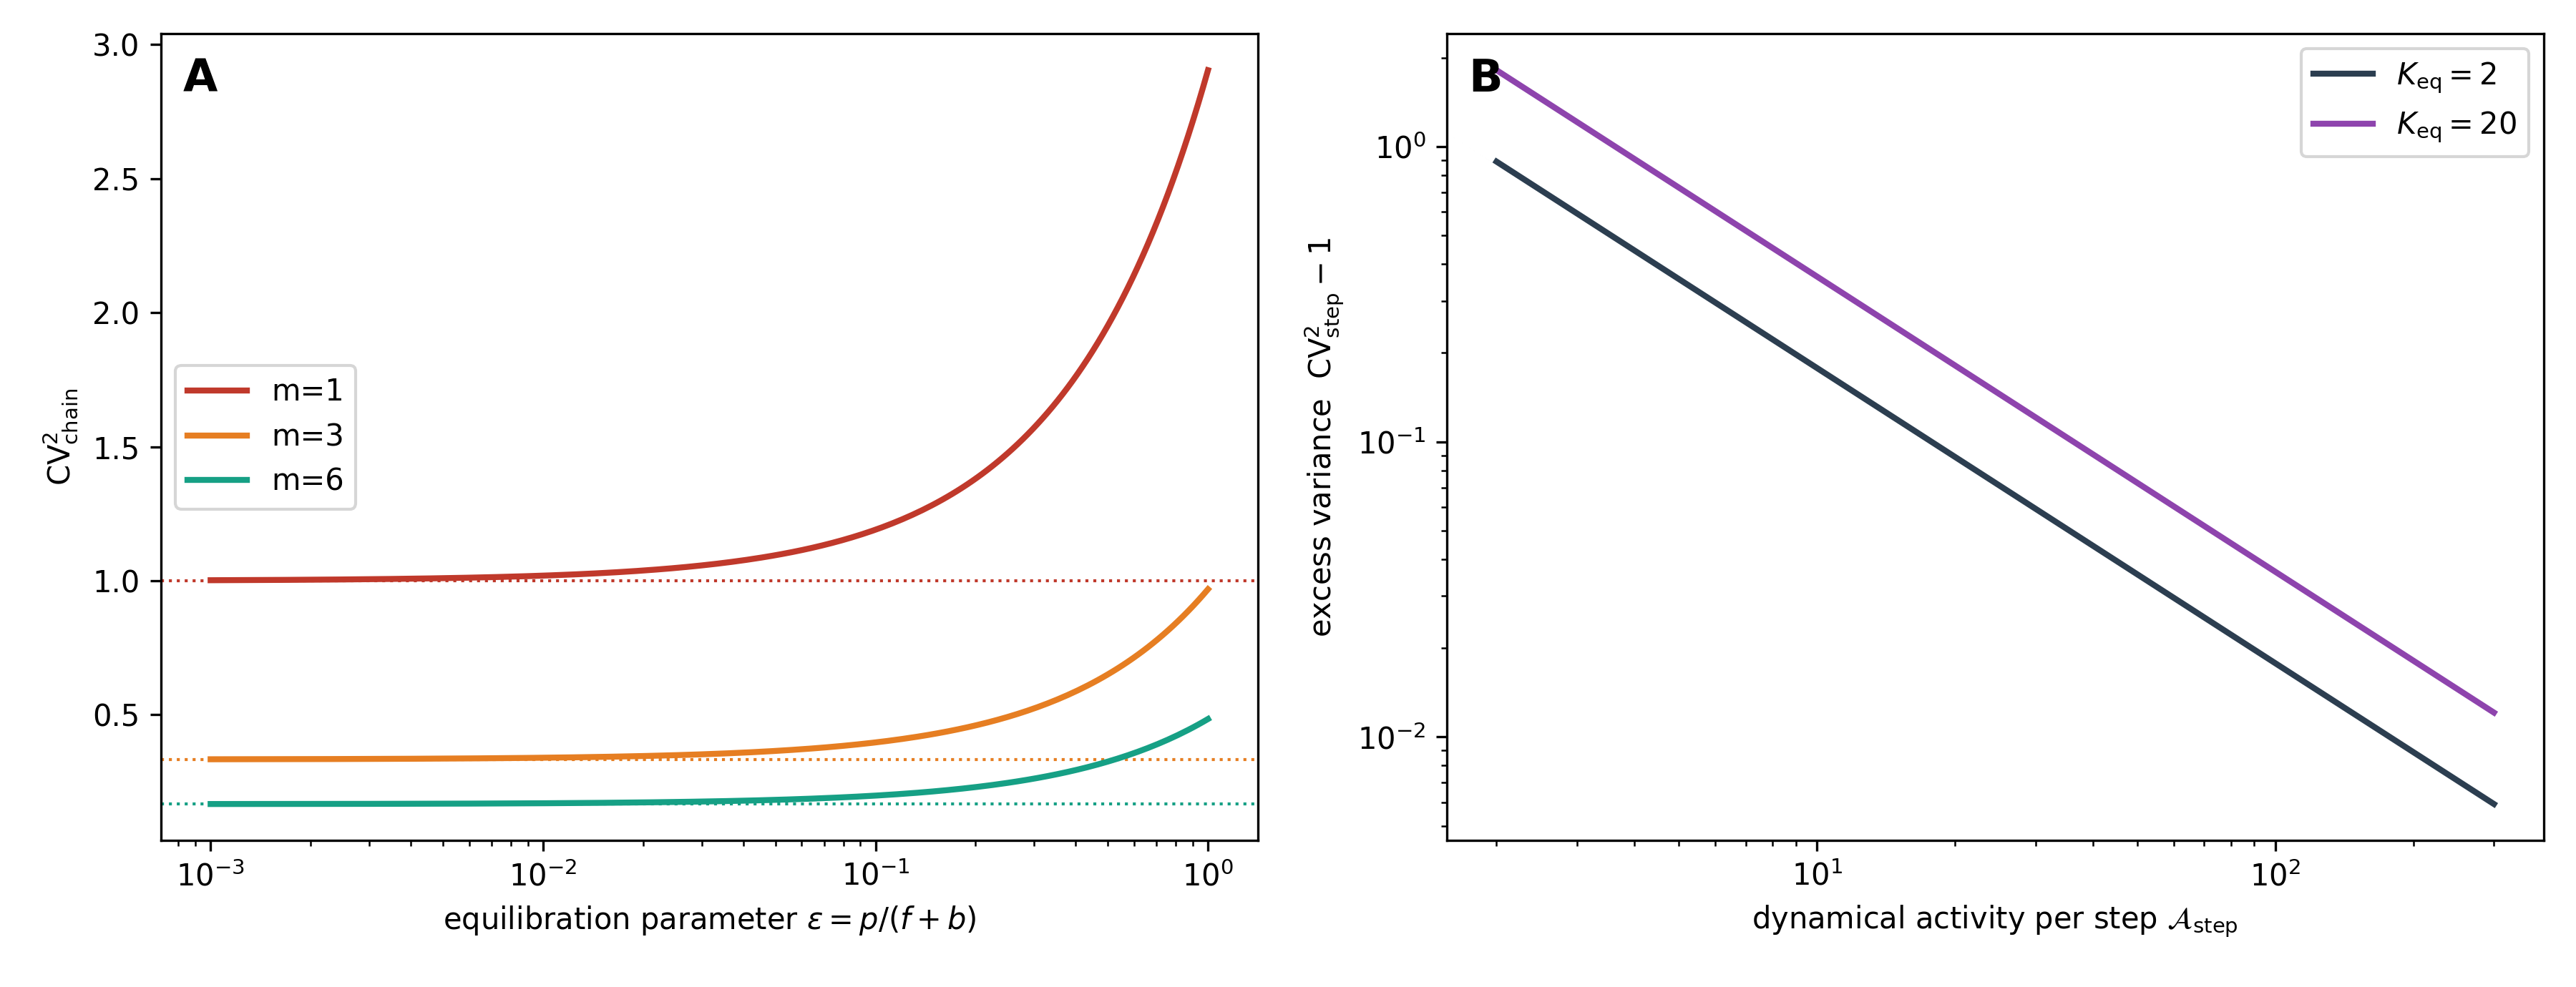
\includegraphics[width=\linewidth]{../figures/fig4_finite.png}
\caption{\textbf{Finite-equilibration correction.} \textbf{(A)} $\CV^2_{\mathrm{chain}}=\tfrac1m(1+2\epsilon\Keq/(1+\Keq))\to 1/m$ (dotted floors) as the equilibration parameter $\epsilon=p/(f+b)\to0$, for $m=1,3,6$ (fixed $\Keq=20$). \textbf{(B)} The exact activity identity $(\CV^2_{\mathrm{step}}-1)\,\Aact_{\mathrm{step}} = 4\Keq^2/(1+\Keq)^2$, shown as excess variance versus dynamical activity per step $\Aact_{\mathrm{step}}$ for two occupancy ratios $\Keq$. Here $\Keq=f/b$ is the trap occupancy ratio and $\Aact_{\mathrm{step}}$ the directed trap traversals per completed step---distinct quantities.}
\label{fig:finite}
\end{figure}

\begin{result}[Residual cost as activity, in this construction]
\label{res:activity}
For the two-state entropic gate, the approach of the compensating chain to its $1/m$ coherence floor is governed by the exact identity~\eqref{eq:activity}; the residual cost appears as dynamical activity---a genuine physical resource, distinct from entropy production---rather than as increased dissipation. We do not claim this identity for arbitrary mechanisms.
\end{result}

\section{Optimality: an Aldous--Shepp sandwich}
\label{sec:sandwich}

We now bound the minimum $\CV^2$ of a \emph{compensating} dwell at fixed internal complexity. We first specify the admissible class and the constraint precisely.

\begin{definition}[Admissible compensating dwell]
\label{def:class}
An \emph{order-$n$ Arrhenius phase-type dwell} is the absorption time of a continuous-time Markov chain on $n$ transient states with a single absorbing exit, entered at a fixed state (initial distribution $\alpha=e_1$), whose transition rates are Arrhenius, $k=A\,\ee^{-E/T}$, with arbitrary prefactors $A>0$ and activation energies $E\in[0,\Emax]$. The topology is arbitrary (reversible, irreversible, or branched) within this class. The \emph{required sensitivity} is $R\equiv\dd\ln\mu/\dd T\big|_{\Tzero}$, where $\mu$ is the mean absorption time; \emph{compensation} means $R>0$ (a period-lengthening dwell, equivalently one that offsets a fixed background negative sensitivity of the remaining cycle). Because $\CV^2$ is invariant under a uniform rescaling of all rates, fixing the mean is immaterial; the optimization is over $\CV^2$ at fixed $R$, over prefactors and activation energies subject to $E\le\Emax$.
\end{definition}

\begin{theorem}[Coherence cost of compensation]
\label{thm:sandwich}
Fix the order $n$ and a required sensitivity $R$ within the range attained by the one-trap construction, $R \le \Emax/[(n-1)\Tzero^2]$. Over the admissible class of Definition~\ref{def:class},
\begin{equation}
\frac{1}{n} \;\le\; \CV^2_{\min}(n,R) \;\le\; \frac{1}{n-1}.
\end{equation}
The lower bound is the Aldous--Shepp theorem \cite{AldousShepp1987}: the least variable order-$n$ phase-type distribution is Erlang, with $\CV^2=1/n$; it holds for every order-$n$ phase-type dwell irrespective of $R$, hence a fortiori under compensation. The upper bound is achieved by the explicit single-entropic-trap construction of Appendix~\ref{app:A7}. Consequently the coherence cost of temperature compensation is at most one effective step and vanishes relative to the ceiling as $n\to\infty$: $\CV^2_{\min}/(1/n)\to 1$.
\end{theorem}

\begin{proof}[Proof sketch]
Lower bound: Aldous--Shepp \cite{AldousShepp1987} applied to Definition~\ref{def:class}. The Erlang minimizer itself cannot compensate by Proposition~\ref{prop:positivity} (its control coefficients are all negative), but the theorem uses only the universal lower bound $\CV^2\ge 1/n$; whether the constrained infimum is separated from $1/n$ for fixed $R$ is part of the extremal problem. Upper bound: the construction of Appendix~\ref{app:A7} uses an $(n-1)$-stage Erlang chain plus one entropic trap on the first stage; equal stage means give $\CV^2=\tfrac{1}{n-1}+\tfrac{2\epsilon\Keq}{(1+\Keq)(n-1)^2}\to\tfrac{1}{n-1}$ as $\epsilon\to0$, valid while $R\le\Emax/[(n-1)\Tzero^2]$. \end{proof}

Constrained optimization (protocol in Appendix~\ref{app:A8}) finds an audited numerical candidate strictly inside the band and nearer the floor (e.g.\ $\CV^2\approx0.426$ at $n=3$, $R=2$, versus $[1/3,\,1/2]$; Fig.~\ref{fig:sandwich}). This candidate is an upper-bound point, not a certificate of global optimality. Closing the sandwich---the exact $\CV^2_{\min}(n,R)$ over Definition~\ref{def:class}---is the central open problem. Its structural (non-moment) nature is why a Lagrangian over moment constraints does not close it: the constraint is membership in the order-$n$ phase-type class, exactly the ingredient that makes the unconstrained problem the nontrivial Aldous--Shepp theorem rather than a moment calculation.

\begin{figure}[t]
\centering
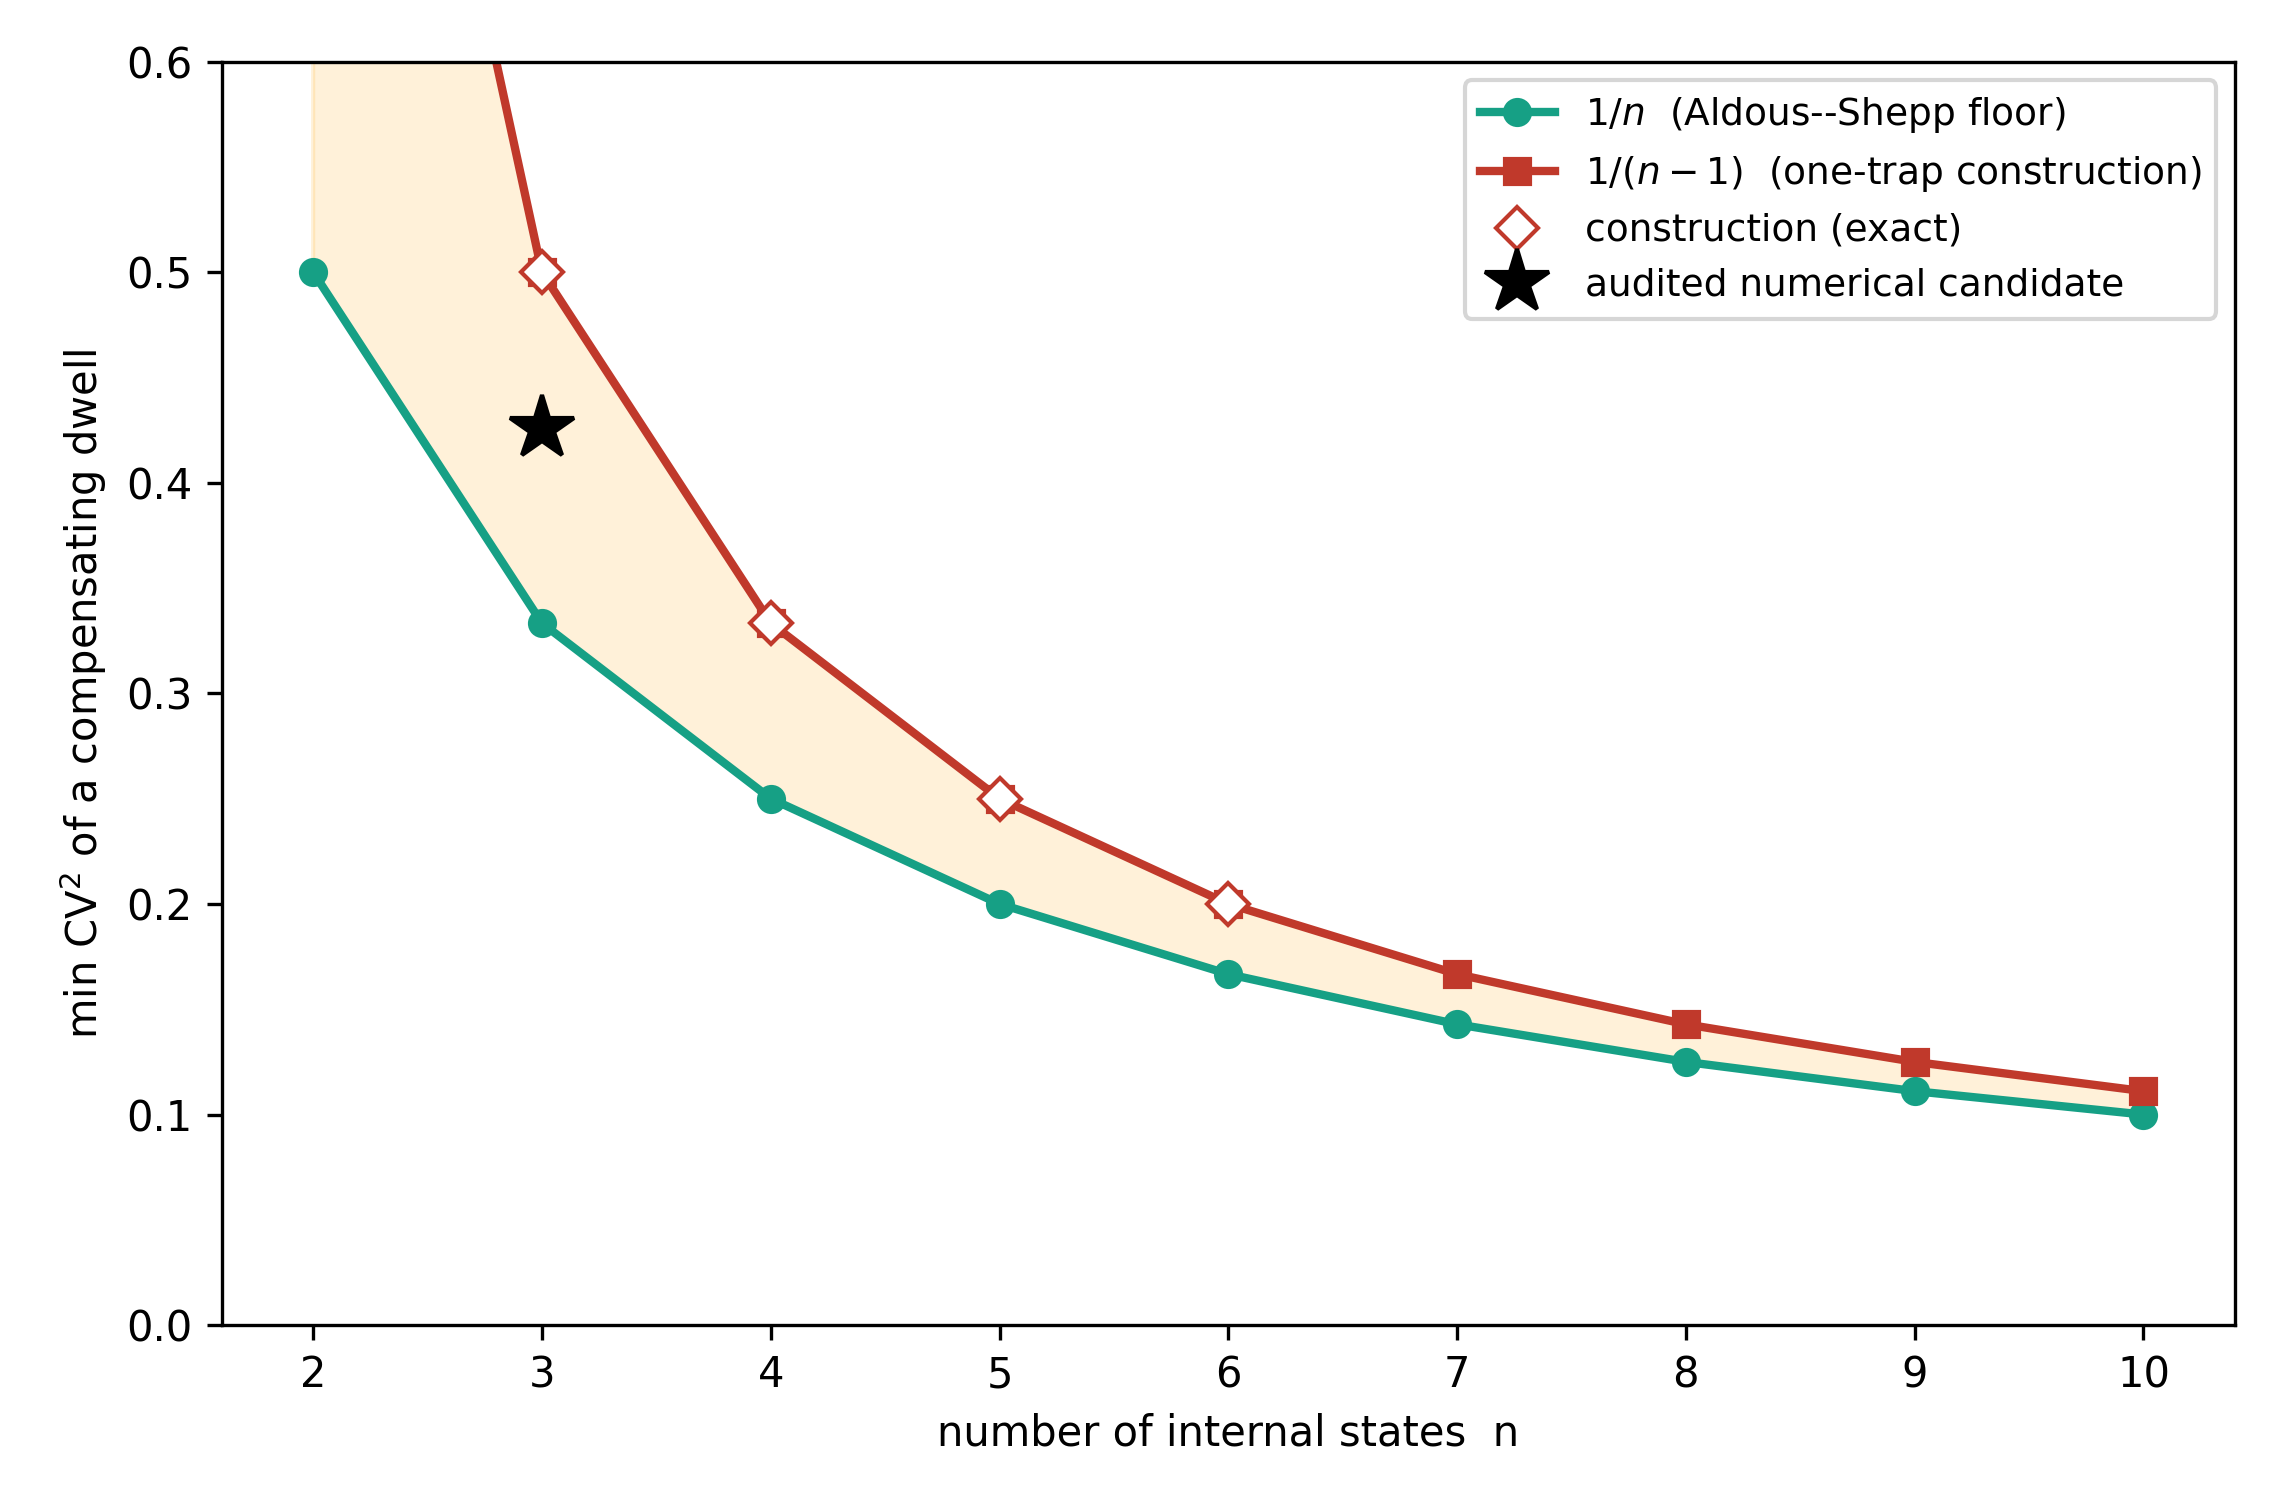
\includegraphics[width=0.7\linewidth]{../figures/fig5_sandwich.png}
\caption{\textbf{The coherence cost of compensation is sandwiched} between the Aldous--Shepp floor $1/n$ (rigorous lower bound) and the one-trap construction $1/(n-1)$ (achievable upper bound). Open diamonds: exact first-passage $\CV^2$ of the construction. Star: audited numerical candidate at $n=3,\,R=2$ (Definition~\ref{def:class}; protocol in Appendix~\ref{app:A8}), strictly interior and interpreted as an upper-bound point rather than a certified global optimum. The cost is less than one effective step and vanishes relative to the ceiling as $n\to\infty$.}
\label{fig:sandwich}
\end{figure}

\section{Discussion}
\label{sec:discussion}

Across three candidate currencies, only one invariant survives. The dissipation cost reported for kinetic-regulation TC \cite{Fu2024} is mechanism-dependent and was negative in our minimal model (Fig.~\ref{fig:trade}C). The precision (coherence) cost is real only for the canonical single-timescale mechanism (Result~\ref{res:single}) and dissolves with internal structure (Result~\ref{res:nofloor}). What remains mechanism-independent is solely the kinematic necessity of a period-lengthening reaction (Proposition~\ref{prop:positivity}, consistent with \cite{Ruoff1992,Fu2024}). The costs of compensating \emph{well} are structural---internal states and an activation-energy contrast $\Emax\ge RT^2$---and kinetic---dynamical activity, governed within the two-state gate by the exact identity~\eqref{eq:activity}, in the spirit of the kinetic uncertainty relation \cite{DiTerlizzi2019,Hiura2021}---and, within the sensitivity range of the explicit construction, are bounded to within a factor $n/(n-1)$ of free (Theorem~\ref{thm:sandwich}).

We emphasize the scope. ``Not entropy production'' is a statement about steady-state dissipation, the quantity bounded in \cite{Fu2024,BaratoSeifert2016}; dynamical activity is itself a physical resource in stochastic thermodynamics, and the residual cost we identify is real, not zero. The precise claim is that, in the model classes analyzed, compensation need not increase entropy production, and the remaining cost appears as internal-state complexity and dynamical activity. Temperature robustness and precision are not fundamentally in tension.

This yields a falsifiable architectural prediction: a clock that is simultaneously precise and well temperature-compensated should implement compensation as a \emph{multi-state}, entropically-gated module---an entropically stabilized, enthalpically costly off-pathway state at each of several stages---rather than a single competing reaction. This is consistent with the cyanobacterial exemplar, whose rate-limiting KaiC ATPase is a large, multi-subunit, multi-conformational enzyme with atomic-scale, entropically complex origins of slowness \cite{Abe2015}, nearly temperature-invariant turnover that sets the period \cite{Terauchi2007}, and a reconstituted rhythm that is both precise and compensated \cite{Nakajima2005}. Concrete tests are collected in Table~\ref{tab:predictions}.

\begin{table}[t]
\centering
\small
\caption{Experimental predictions. Each row is a discriminating observation between the single-timescale regime (Result~\ref{res:single}) and the entropic-gating regime (Results~\ref{res:nofloor}--\ref{res:activity}).}
\label{tab:predictions}
\begin{tabular}{L{5.2cm} L{4.6cm} L{4.0cm}}
\toprule
\textbf{Prediction} & \textbf{Observable} & \textbf{System} \\
\midrule
A single competing-delay module should show a compensation--precision trade-off & period CV$^2$ rises as compensation is approached & synthetic oscillator / minimal biochemical loop \\
\addlinespace
Multi-state entropic gates preserve precision under compensation & period CV$^2$ stays near the Erlang floor $1/m$ & KaiC mutants / engineered gated enzymes \\
\addlinespace
Disrupting fast trap equilibration raises timing noise without necessarily raising dissipation & CV$^2$ increases at fixed period; entropy production not increased & KaiC conformational mutants \\
\addlinespace
Compensation strength scales with the activation/enthalpy contrast of the off-pathway state & shift in temperature sensitivity $R$ with $\Delta H$ & mutational perturbation of an off-pathway state \\
\bottomrule
\end{tabular}
\end{table}

Two directions would complete the theory. First, the finite-equilibration law~\eqref{eq:finiteeps} and activity identity~\eqref{eq:activity} should be promoted from the two-state gate to a one-sided bound over all mechanisms, connecting the residual cost to activity as in first-passage kinetic uncertainty relations \cite{Garrahan2017,Hiura2021}. Second, the exact constrained optimum of Theorem~\ref{thm:sandwich}---the minimum $\CV^2$ over order-$n$ phase-type dwells subject to $R>0$ (Definition~\ref{def:class})---remains open; Aldous--Shepp \cite{AldousShepp1987} solved the unconstrained version, and the compensation constraint reopens it as a clean extremal-phase-type problem whose solution would pin the coherence cost of temperature compensation exactly.

\paragraph{Data and code availability.} A complete reproducibility package accompanies this manuscript (Python library, one script per figure, a cached and audited numerical candidate for Fig.~\ref{fig:sandwich}, and a \texttt{pytest} suite that asserts the exact analytic identities of Eqs.~\eqref{eq:trapmoments}--\eqref{eq:activity} and the bounds of Theorem~\ref{thm:sandwich}). All figures and the deterministic audit of the constrained-optimization candidate in Appendix~\ref{app:A8} are regenerated by it. Repository DOI: \texttt{[to be added]}.

\appendix
\section{Derivations and numerical protocols}
\label{app:derivations}

Throughout, first-passage moments of an $n$-state absorbing chain with transient sub-generator $Q$ (row convention; exit rates are the negative row sums) are computed from the fundamental matrix $\mathcal{F}=(-Q)^{-1}$ via $m_1=(\mathcal{F}\mathbf 1)_{\mathrm{entry}}$ and $m_2=2(\mathcal{F}^2\mathbf 1)_{\mathrm{entry}}$, with variance $v=m_2-m_1^2$ \cite{Neuts1981,Cox1962}.

\subsection{Node-0 waiting time}
\label{app:A1}
At node $0$ the walker waits an exponential time (rate $a+d$), then with probability $a/(a+d)$ advances (contributing that wait only) or with probability $d/(a+d)$ performs an excursion (Laplace transform $\psi_e$) and returns to node $0$, restarting the dwell. The renewal equation $\psi_0(s)=\tfrac{a+d}{a+d+s}\bigl[\tfrac{a}{a+d}+\tfrac{d}{a+d}\psi_e(s)\psi_0(s)\bigr]$ solves to Eq.~\eqref{eq:psi0}.

\subsection{Cycle mean and variance}
\label{app:A2}
With exponential excursion $\psi_e(s)=\gamma/(\gamma+s)$, $\mu_e=1/\gamma$, expanding $\psi_0$ about $s=0$ gives node-0 mean $1+\Delta$ and variance $1+2\Delta+2\mu_e\Delta+\Delta^2$ ($\Delta=n_{\mathrm{ex}}\mu_e$, $n_{\mathrm{ex}}=d/a$, units $a=1$). Adding $N-1$ exponential ring stages (each mean and variance $1$) gives $\tau=N+\Delta$ and $\mathrm{Var}=N+2\Delta+2\mu_e\Delta+\Delta^2$. (Verified symbolically; see reproducibility package.)

\subsection{Compensation condition}
\label{app:A3}
With Arrhenius temperature dependence, ring-stage dwell times scale as $\ee^{E_A/T}$. The side-excursion delay scales as $\ee^{(E_A+E_e-E_B)/T}$. Hence
\begin{equation}
\frac{\dd\tau}{\dd T}=-\frac{1}{T^2}
\left[N E_A+(E_A+E_e-E_B)\Delta\right],
\end{equation}
and $\dd\tau/\dd T=0$ gives $\Delta^\ast=NE_A/G$ with $G=E_B-E_A-E_e>0$.

\subsection{Compensated coherence}
\label{app:A4}
In the low-variance limit $\mu_e\to0$ at fixed $\Delta$, $\mathrm{Var}\to N+2\Delta+\Delta^2$, so $\Ncoh=\tau^2/(\pi\mathrm{Var})=(N+\Delta)^2/[\pi(N+2\Delta+\Delta^2)]$; substituting $\Delta=\Delta^\ast$ gives Eq.~\eqref{eq:frontier}. Limits: $\Delta^\ast\to0$ ($G\to\infty$) gives $N/\pi$; $\Delta^\ast\to\infty$ ($G\to0^+$) gives $1/\pi$.

\subsection{Gated-chain floor}
\label{app:A5}
A fast-equilibrating pool $X\rightleftharpoons Y$ with slow exit is, to leading order in $\epsilon=p/(f+b)$, an exponential stage of rate $k_{\mathrm{eff}}=p/(1+\Keq)$; $m$ such stages in series form an Erlang-$m$ dwell with $\CV^2\to1/m$. The temperature sensitivity enters only through $\Keq(T)$ and is independent of $m$, giving Result~\ref{res:nofloor}.

\subsection{Single gated step}
\label{app:A6}
For the two-state sub-generator $-Q=\bigl(\begin{smallmatrix}p+f & -f\\ -b & b\end{smallmatrix}\bigr)$, $\det(-Q)=pb$ and $\mathcal{F}=(pb)^{-1}\bigl(\begin{smallmatrix}b & f\\ b & p+f\end{smallmatrix}\bigr)$. Hence $m_1=(1+\Keq)/p$ ($\Keq=f/b$) and $\CV^2_{\mathrm{step}}=1+2fp/(b+f)^2=1+2\epsilon\Keq/(1+\Keq)$ with $\epsilon=p/(f+b)$; for $m$ independent stages $\CV^2_{\mathrm{chain}}=\CV^2_{\mathrm{step}}/m$. The expected time in $X$ before absorption is $\mathcal{F}_{00}=1/p$, so the expected numbers of $X\!\to\!Y$ and $Y\!\to\!X$ traversals are each $f/p$, giving directed activity $\Aact_{\mathrm{step}}=2f/p=2\Keq/[\epsilon(1+\Keq)]$. Then $(\CV^2_{\mathrm{step}}-1)\Aact_{\mathrm{step}}=4\Keq^2/(1+\Keq)^2$.

\subsection{One-trap construction}
\label{app:A7}
Take an $(n-1)$-stage forward chain and attach a single entropic trap ($X_0\rightleftharpoons Y$) to the first stage, $n$ states total. Setting the plain-stage rates to $p_1/(1+\Keq)$ makes all $n-1$ stages have equal mean; the trapped stage contributes variance $\CV^2_{\mathrm{step}}\mu^2$ and the rest $\mu^2$ each, giving $\CV^2=\tfrac{n-2+\CV^2_{\mathrm{step}}}{(n-1)^2}=\tfrac{1}{n-1}+\tfrac{2\epsilon\Keq}{(1+\Keq)(n-1)^2}\to\tfrac1{n-1}$ as $\epsilon\to0$. The single trap supplies the anomalous sensitivity; with plain-stage activation energies set to zero, the attainable $R$ is $\le\Emax/[(n-1)T^2]$.

\subsection{Constrained-optimization protocol}
\label{app:A8}
For fixed $n$ we parametrize all $n(n-1)$ transient--transient rates and $n$ exit rates as $A_{ij}=\ee^{x_{ij}}$, $E_{ij}=\Emax\,\sigma(y_{ij})$ (logistic $\sigma$, enforcing $E\in[0,\Emax]$), and minimize $\CV^2(\mathbf x,\mathbf y)$ at $\Tzero=1$ subject to the equality constraint $R(\mathbf x,\mathbf y)=R_{\mathrm{target}}$ (SLSQP, multi-start). Each candidate optimum is re-audited: $R$ is recomputed by central differences at three step sizes $\dd T\in\{10^{-2},3\!\times\!10^{-3},10^{-3}\}$ and rejected unless the estimates agree to within $5\%$ and match $R_{\mathrm{target}}$ to $0.06$. This rejects numerically unstable (near-degenerate) candidates. The reproducibility package stores the accepted $n=3$, $R=2$ candidate as a JSON file and verifies it deterministically; the reported value is therefore an audited upper-bound point for $\CV^2_{\min}(n,R)$, not a certificate of global optimality.

\begin{thebibliography}{99}

\bibitem{Nakajima2005} M. Nakajima, K. Imai, H. Ito, T. Nishiwaki, Y. Murayama, H. Iwasaki, T. Oyama, and T. Kondo, \emph{Reconstitution of circadian oscillation of cyanobacterial KaiC phosphorylation in vitro}, Science \textbf{308}, 414--415 (2005).

\bibitem{Terauchi2007} K. Terauchi, Y. Kitayama, T. Nishiwaki, K. Miwa, Y. Murayama, T. Oyama, and T. Kondo, \emph{ATPase activity of KaiC determines the basic timing for circadian clock of cyanobacteria}, Proc. Natl. Acad. Sci. USA \textbf{104}, 16377--16381 (2007).

\bibitem{Ruoff1992} P. Ruoff, \emph{Introducing temperature-compensation in any reaction kinetic oscillator model}, J. Interdiscipl. Cycle Res. \textbf{23}, 92--99 (1992).

\bibitem{Wu2017} L. Wu, Q. Ouyang, and H. Wang, \emph{Robust network topologies for generating oscillations with temperature-independent periods}, PLoS ONE \textbf{12}, e0171263 (2017).

\bibitem{RuoffWesterhoff2007} P. Ruoff, M. Zakhartsev, and H. V. Westerhoff, \emph{Temperature compensation through systems biology}, FEBS J. \textbf{274}, 940--950 (2007).

\bibitem{Fu2024} H. Fu, C. Fei, Q. Ouyang, and Y. Tu, \emph{Temperature compensation through kinetic regulation in biochemical oscillators}, Proc. Natl. Acad. Sci. USA \textbf{121}, e2401567121 (2024).

\bibitem{BaratoSeifert2017} A. C. Barato and U. Seifert, \emph{Coherence of biochemical oscillations is bounded by driving force and network topology}, Phys. Rev. E \textbf{95}, 062409 (2017).

\bibitem{Oberreiter2022} L. Oberreiter, U. Seifert, and A. C. Barato, \emph{Universal minimal cost of coherent biochemical oscillations}, Phys. Rev. E \textbf{106}, 014106 (2022).

\bibitem{Cao2015} Y. Cao, H. Wang, Q. Ouyang, and Y. Tu, \emph{The free-energy cost of accurate biochemical oscillations}, Nat. Phys. \textbf{11}, 772--778 (2015).

\bibitem{Fei2018} C. Fei, Y. Cao, Q. Ouyang, and Y. Tu, \emph{Design principles for enhancing phase sensitivity and suppressing phase fluctuations simultaneously in biochemical oscillatory systems}, Nat. Commun. \textbf{9}, 1434 (2018).

\bibitem{BaratoSeifert2016} A. C. Barato and U. Seifert, \emph{Cost and precision of Brownian clocks}, Phys. Rev. X \textbf{6}, 041053 (2016).

\bibitem{DiTerlizzi2019} I. Di Terlizzi and M. Baiesi, \emph{Kinetic uncertainty relation}, J. Phys. A: Math. Theor. \textbf{52}, 02LT03 (2019).

\bibitem{Hiura2021} K. Hiura and S.-i. Sasa, \emph{Kinetic uncertainty relation on first-passage time for accumulated current}, Phys. Rev. E \textbf{103}, L050103 (2021).

\bibitem{Garrahan2017} J. P. Garrahan, \emph{Simple bounds on fluctuations and uncertainty relations for first-passage times of counting observables}, Phys. Rev. E \textbf{95}, 032134 (2017).

\bibitem{BaratoSeifert2015} A. C. Barato and U. Seifert, \emph{Thermodynamic uncertainty relation for biomolecular processes}, Phys. Rev. Lett. \textbf{114}, 158101 (2015).

\bibitem{Gingrich2016} T. R. Gingrich, J. M. Horowitz, N. Perunov, and J. L. England, \emph{Dissipation bounds all steady-state current fluctuations}, Phys. Rev. Lett. \textbf{116}, 120601 (2016).

\bibitem{Neuts1981} M. F. Neuts, \emph{Matrix-Geometric Solutions in Stochastic Models: An Algorithmic Approach} (Johns Hopkins University Press, Baltimore, 1981).

\bibitem{Cox1962} D. R. Cox, \emph{Renewal Theory} (Methuen, London, 1962).

\bibitem{AldousShepp1987} D. Aldous and L. Shepp, \emph{The least variable phase type distribution is Erlang}, Stochastic Models \textbf{3}, 467--473 (1987).

\bibitem{Abe2015} J. Abe \emph{et al.}, \emph{Atomic-scale origins of slowness in the cyanobacterial circadian clock}, Science \textbf{349}, 312--316 (2015).

\end{thebibliography}

\end{document}
